%Este trabalho está licenciado sob a Licença Atribuição-CompartilhaIgual 4.0 Internacional Creative Commons. Para visualizar uma cópia desta licença, visite http://creativecommons.org/licenses/by-sa/4.0/deed.pt_BR ou mande uma carta para Creative Commons, PO Box 1866, Mountain View, CA 94042, USA.

\chapter{EDO linear de ordem mais alta com coeficientes variáveis}\label{cap_edolcv}
\thispagestyle{fancy}

Neste capítulo, ...

\section{EDO de ordem 2 com coeficientes variáveis: fundamentos}\label{cap_edolcv_sec_edo2lcvfun}

Nesta seção, vamos discutir de forma bastante introdutória o caso de EDOs lineares de ordem 2 com coeficientes não constantes, i.e. EDOs da forma
\begin{equation}
  p(x)y'' + q(x)y' + r(x)y = g(x),
\end{equation}
sendo $y = y(x)$ e $p(x)\not\equiv 0$.

A teoria fundamental para tais equações é análoga a de equações com coeficientes constantes. Mais precisamente, a solução geral pode ser escrita na forma
\begin{equation}
  y(t) = c_1y_1(x) + c_2y_2(x) + y_p(x),
\end{equation}
onde $y_1$ e $y_2$ formam um conjunto de soluções fundamentais ($W(y_1,y_2;t)\neq 0$) para a equação homogênea associada e $y_p$ é uma solução particular da equação não homogênea. Cabe observar que a existência e unicidade de solução (para um PVI com equação homogênea) é garantida quando os coeficientes $p$, $q$ e $r$ são funções contínuas no domínio de interesse.

A seguir, vamos explorar dois casos. O primeiro, é a \emph{equação de Euler}\footnote{Leonhard Euler, 1707-1783, matemático suíço. Fonte: \href{https://en.wikipedia.org/wiki/Leonhard_Euler}{Wikipedia}.}, a qual admite soluções da forma $y = x^r$ e pode ser tratada usando as mesmas abordagem utilizadas no caso das equações com coeficientes constantes. O segundo caso, são de equações que admitem \emph{soluções em série de potências}.

\subsection{Equação de Euler}

Um caso fundamental de uma EDO linear de segunda ordem com coeficientes não constantes é a \emph{equação de Euler}
\begin{equation}
  {\color{blue}x^2y'' + axy' + by = 0},
\end{equation}
onde $a,b$ são constantes e $y = y(x)$.

Assumindo uma solução da forma
\begin{equation}
  {\color{blue}y(t) = x^r}
\end{equation}
e substituindo na EDO, obtemos
\begin{equation}
  x^2r(r-1)x^{r-2} + axrx^{r-1} + bx^r = 0.
\end{equation}
Rearranjando os termos, temos a \emph{equação característica}
\begin{equation}
  r(r-1) + ar + b = 0
\end{equation}
ou, equivalentemente,
\begin{equation}
  {\color{blue}r^2 + (a-1)r + b = 0}.
\end{equation}
Suas raízes são
\begin{equation}
  r_1, r_2 = \frac{(1-a)\pm\sqrt{(a-1)^2-4b}}{2}.
\end{equation}

\subsubsection{Raízes reais distintas}

No caso de $(a-1)^2-4b\neq 0$, temos que as raízes $r_1$ e $r_2$ da equação característica são reais e distintas ($r_1\neq r_2$). Assim, $y_1(x) = x^{r_1} $ e $y_2(x) = x^{r_2}$ são soluções da equação de Euler e o wronskiano
\begin{align}
  W(y_1,y_2;t) &=
                 \begin{vmatrix}
                   y_1 & y_2 \\
                   y_1' & y_2'
                 \end{vmatrix} \\
               &=
                 \begin{vmatrix}
                   x^{r_1} & x^{r_2} \\
                   r_1x^{r_1-1} & r_2x^{r_2-1}
                 \end{vmatrix} \\
               &= (r_2-r_1)x^{r_1+r_2-1} \neq 0.\\
\end{align}
Ou seja, $\{y_1,y_2\}$ formam um conjunto fundamental de soluções para a equação de Euler, logo sua \emph{solução geral} é
\begin{equation}
  {\color{blue}y(t) = c_1x^{r_1} + c_2x^{r_2}}.
\end{equation}

\begin{ex}
  Vamos encontrar a solução geral de
  \begin{equation}
    x^2y'' + xy -4y = 0.
  \end{equation}

  Supondo uma solução da forma $y(t) = x^r$, obtemos a equação característica associada
  \begin{equation}
    r^2 - 4 = 0.
  \end{equation}
  Suas raízes são $r_1 = -2$ e $r_2 = 2$. Logo, concluímos que a solução geral é
  \begin{equation}
    y(x) = c_1x^{-2} + c_2x^2.
  \end{equation}

  \ifispython
  No \python\footnote{Veja Observação \ref{obs:cap_edolin_python}}, temos
\begin{verbatim}
>>> dsolve(x**2*diff(y(x),x,2)+x*diff(y(x),x)-4*y(x))
Eq(y(x), C1/x**2 + C2*x**2)
\end{verbatim}
  \fi
\end{ex}

\subsubsection{Raiz dupla}

No caso de $(a-1)^2-4b = 0$, a equação característica tem raiz dupla
\begin{equation}
  r = \frac{1-a}{2}.
\end{equation}
Isto nos fornece a solução particular
\begin{equation}
  y_1(t) = x^r.
\end{equation}
Para obtermos uma outra solução, usamos o \emph{método da redução de ordem}. I.e., buscamos por uma solução da forma
\begin{equation}
  y_2(x) = u(x)y_1(x),
\end{equation}

Substituindo $y_2$ na equação de Euler, obtemos
\begin{align}
  0 &= x^2y_2'' + axy_2' + by_2 \\
    &= x^2\left(y_1''u + 2y_1'u' + y_1u''\right) \\
    &+ ax\left(y_1'u + y_1u'\right) \\
    &+ by_1u \\
    &= \underbrace{\left(x^2y_1'' + axy_1' + By_1\right)u}_{=0} \\
    &+ x^2y_1u'' + (2x^2y_1' + axy_1)u' \\
    &= x^{r+2}u'' + (2x^2rx^{r-1} + axx^r)u' \\
    &= x^{r+2}u'' + (2r+a)x^{r+1}u' \\
    &= x^{r+2}u'' + x^{r+1}u' 
\end{align}
Desta equação, obtemos
\begin{align}
  x^{r+2}u'' = -x^{r+1}u' &\Rightarrow \frac{1}{u'}u'' = -x^{-1} \\
                                &\Rightarrow \ln|u'| = -\ln|x| + c \\
                          &\Rightarrow u' = \frac{c}{x} \\
                          &\Rightarrow u = c\ln|x| + d.
\end{align}
Ou seja, podemos escolher $y_2(x) = x^r\ln|x|$. Conferindo o wronskiano, temos
\begin{align}
  W(y_1,y_2;t) &=
  \begin{vmatrix}
    x^r & x^r\ln|x| \\
    rx^{r-1} & (r\ln|x| + 1)x^{r-1}
  \end{vmatrix} \\
        &= x^{2r-1} \neq 0,\quad x\neq 0.
\end{align}
Concluímos que, no caso de raiz dupla $r=(1-a)/2$, a solução geral da equação de Euler é
\begin{equation}
  y(t) = (c_1 + c_2\ln|x|)x^{\frac{1-a}{2}}.
\end{equation}

\begin{ex}
  Vamos obter a solução geral de
  \begin{equation}
    x^2y'' - xy' + y = 0.
  \end{equation}

  A equação característica associada é
  \begin{equation}
    r^2 -2r + 1 = 0,
  \end{equation}
  a qual tem raiz dupla $r = 1$. Logo, a solução geral desta equação de Euler é
  \begin{equation}
    y(t) = (c_1 + c_2\ln|x|)x.
  \end{equation}

  \ifispython
  No \python\footnote{Veja Observação \ref{obs:cap_edolin_python}}, temos
\begin{verbatim}
>>> dsolve(x**2*diff(y(x),x,2)-x*diff(y(x),x)+y(x))
Eq(y(x), x*(C1 + C2*log(x)))
\end{verbatim}
  \fi  
\end{ex}

\subsubsection{Raízes complexas}

No caso de $(a-1)^2-4b < 0$, a equação característica associada a equação de Euler tem raízes complexas
\begin{equation}
  r_1,r_2 = \lambda \pm i\mu
\end{equation}
onde
\begin{equation}
  \lambda = \frac{(1-a)}{2}\quad\text{e}\quad \mu = \frac{\sqrt{4b - (a-1)^2}}{2}.
\end{equation}
Da \emph{fórmula de Euler}, temos
\begin{align}
  x^{\lambda\pm i\mu} &= e^{\ln x^{\lambda \pm i\mu}} \\
                      &= e^{(\lambda \pm i\mu)\ln(x)} \\
                      &= e^{\lambda\ln|x|}[\cos(\mu\ln x) \pm i\sen(\mu\ln x)] \\
                      &= x^\lambda[\cos(\mu\ln x) \pm i\sen(\mu\ln x)].
\end{align}
Agora, da linearidade da equação de Euler, vemos que $y_1(x) = x^\lambda\cos(\mu\ln|x|)$ e $y_2(x) = x^\lambda\sen(\mu\ln|x|)$ são soluções particulares. Mais ainda, o wronskiano
\begin{align}
  W(y_1,y_2;t) &=
                 \begin{vmatrix}
                   y_1 & y_2 \\
                   y_1' & y_2'
                 \end{vmatrix} \\
               &= \mu x^{2\lambda-1} \\
               &= \frac{\sqrt{4b-(a-1)^2}}{2}x^a \neq 0.
\end{align}
Concluímos que, no caso de raiz dupla, a solução geral é
\begin{equation}
  y(t) = x^\lambda[c_1\cos(\mu\ln|x|) + c_2\sen(\mu\ln|x|)].
\end{equation}

\begin{ex}
  Vamos obter a solução geral de
  \begin{equation}
    x^2y'' + xy' + y = 0.
  \end{equation}

  A equação característica associada é
  \begin{equation}
    r^2 + 1 = 0,
  \end{equation}
  a qual tem raízes imaginárias $r = \pm i$. Logo, a solução geral desta equação de Euler é
  \begin{equation}
    y(t) = c_1\cos(\ln|x|) + c_2\sen(\ln|x|).
  \end{equation}

  \ifispython
  No \python\footnote{Veja Observação \ref{obs:cap_edolin_python}}, temos
\begin{verbatim}
>>> dsolve(x**2*diff(y(x),x,2)+x*diff(y(x),x)+y(x))
Eq(y(x), C1*sin(log(x)) + C2*cos(log(x)))
\end{verbatim}
  \fi    
\end{ex}

\subsection{Solução em série de potências}

Em muitos casos, a solução geral de tais EDOs pode ser escrita como uma série de potências, i.e.
\begin{equation}
  y(t) = \sum_{n=0}^{\infty} a_n(x-x_0)^n.
\end{equation}
O ponto $x_0$ é arbitrário e deve pertencer ao domínio de interesse. A ideia básica é, então, substituir a representação em série de potência de $y$ na EDO de forma a calcular seus coeficientes.

\begin{ex}
  Vamos usar o método de série de potências para resolver
  \begin{equation}
    y'' - xy = 0,
  \end{equation}
  chamada \emph{equação de Airy}\footnote{Sir George Biddell Airy, 1801 - 1892, matemático inglês. Fonte: \href{https://en.wikipedia.org/wiki/George_Biddell_Airy}{Wikipedia}.}.

  Vamos assumir que
  \begin{equation}
    y(t) = \sum_{n=0}^{\infty} a_nx^n.
  \end{equation}
  Segue que
  \begin{align}
    y'(t) &= \sum_{n=1}^\infty a_{n}nx^{n-1} \\
          &= \sum_{n=0}^\infty a_{n+1}(n+1)x^n
  \end{align}
  e
  \begin{align}
    y''(t) &= \sum_{n=1}^\infty a_{n+1}(n+1)nx^{n-1} \\
           &= \sum_{n=0}^\infty a_{n+2}(n+2)(n+1)x^n.
  \end{align}
  Substituindo na equação de Airy, obtemos
  \begin{align}
    0 &= y'' - xy \\
      &= \sum_{n=0}^\infty a_{n+2}(n+2)(n+1)x^n - x\sum_{n=0}^\infty a_{n}x^n \\
      &= \sum_{n=0}^\infty a_{n+2}(n+2)(n+1)x^n - \sum_{n=0}^\infty a_{n}x^{n+1} \\
      &= 2a_2 + \sum_{n=1}^\infty a_{n+2}(n+2)(n+1)x^n - \sum_{n=1}^\infty a_{n-1}x^{n} \\
      &= 2a_2 + \sum_{n=1}^\infty (a_{n+2}(n+2)(n+1) - a_{n-1})x^n.
  \end{align}
  Como esta última equação deve valer para todo $x$, segue que
  \begin{align}
    & a_2 = 0, \\
    & (n+2)(n+1)a_{n+2} = a_{n-1},\quad n=1, 2, 3, \ldots
  \end{align}
  Observamos que não há condições impostas para $a_0$ e $a_1$, ou seja, são constantes indeterminadas. Das relações acima, obtemos:
  \begin{enumerate}[a)]
  \item $n = 3, 6, 9, \ldots$:
    \begin{align}
      a_5 &= \frac{a_2}{4\cdot 5} = 0 \\
      a_8 &= \frac{a_5}{7\cdot 9} = 0 \\
      a_{11} &= \frac{a_{8}}{10\cdot 11} = 0 \\
          &\vdots \\
      a_{3k+2} &= 0,\quad k\geq 1.
    \end{align}
  \item $n = 1, 4, 7, \ldots$:
    \begin{align}
      a_3 &= \frac{a_0}{2\cdot 3}, \\
      a_6 &= \frac{a_3}{5\cdot 6} = \frac{a_0}{2\cdot 3\cdot 5\cdot 6}, \\
      a_9 &= \frac{a_{6}}{8\cdot 9} = \frac{a_0}{2\cdot 3\cdot 5\cdot 6 \cdot 8 \cdot 9} \\
          &\vdots \\
      a_{3k} &= \frac{a_0}{2\cdot 3 \cdot\cdots\cdot (3k-1)\cdot (3k)},\quad k\geq 1.
    \end{align}
  \item $n = 2, 5, 8, \ldots$:
    \begin{align}
      a_4 &= \frac{a_1}{3\cdot 4}, \\
      a_7 &= \frac{a_4}{6\cdot 7} = \frac{a_1}{3\cdot 4 \cdot 6 \cdot 7},\\
      a_{10} &= \frac{a_{7}}{9\cdot 10} = \frac{a_1}{3\cdot 4 \cdot 6 \cdot 7\cdot 9 \cdot 10},\\
          &\vdots \\
      a_{3k+1} &= \frac{a_1}{3\cdot 4 \cdot\cdots\cdot (3k)\cdot (3k+1)},\quad k\geq 1.
    \end{align}
  \end{enumerate}
  Do que calculamos, podemos concluir que
  \begin{align}
    y(t) &= a_0\left[1 + \sum_{k=1}^\infty \frac{x^{3k}}{2\cdot 3 \cdot\cdots\cdot (3k-1)\cdot (3k)}\right] \\
         &+ a_1\left[x + \sum_{k=1}^\infty \frac{x^{3k+1}}{3\cdot 4 \cdot\cdots\cdot (3k)\cdot (3k+1)}\right].
  \end{align}
\end{ex}

Há uma série de questões importantes que fogem dos objetivos destas notas de aula. Por exemplo, observamos que nem sempre é possível escrever a solução de uma EDO como uma série de potências. Também deve-se fazer um tratamento especial quando $P(x_0)=0$. Para maiores informações, pode-se consultar \cite{Boyce2017}.

\subsection*{Exercícios resolvidos}

\begin{exeresol}
  Resolva
  \begin{align}
    & x^2y'' - 2xy' + 2y = 0, \\
    & y(1) = 0\quad\text{e}\quad y'(1) = -1.
  \end{align}
\end{exeresol}
\begin{resol}
  Trata-se de um PVI envolvendo a equação de Euler. Primeiramente, buscamos a solução geral desta equação. Para tanto, resolvemos a equação característica associada
  \begin{equation}
    r^2 - 3r + 2 = 0.
  \end{equation}
  As raízes desta equação são
  \begin{equation}
    r_1 = 1\quad\text{e}\quad r_2 = 2.
  \end{equation}
  Logo, a solução geral da EDO é
  \begin{equation}
    y(t) = c_1x + c_2x^2.
  \end{equation}

  Agora, das condições iniciais, obtemos
  \begin{align}
    & y(1) = 0 \Rightarrow c_1 + c_2 = 0 \\
    & y'(1) = -1 \Rightarrow c_1 + 2c_2 = -1
  \end{align}
  Resolvendo, obtemos $c_1=1$ e $c_2=-1$. Concluímos que a solução do PVI é
  \begin{equation}
    y(t) = x - x^2.
  \end{equation}
\end{resol}

\begin{exeresol}
  Considere o seguinte PVI
  \begin{align}
    & y'' + xy' = \cos(x),\\
    & y(0)=1,\quad y'(0)=0.
  \end{align}
  Calcule os quatro primeiros termos da representação da solução em série de potências em torno de $x_0=0$.
\end{exeresol}
\begin{resol}
  Consideramos que a solução possa ser escrita como uma série de potências da forma
  \begin{equation}
    y(x) = \sum_{n=0}^\infty a_nx^n.
  \end{equation}
  Ainda, lembramos que
  \begin{align}
    \cos(x) = \sum_{n=0}^\infty \frac{(-1)^nx^{2n}}{(2n)!}.
  \end{align}
  Assim sendo, substituímos na EDO para encontrarmos
  \begin{align}
    \cos(x) &= y'' + xy' \\
    \sum_{n=0}^\infty \frac{(-1)^nx^{2n}}{(2n)!} &= \sum_{n=0}^\infty a_{n+2}(n+2)(n+1)x^n \\
            &+ x\sum_{n=0}^\infty a_{n+1}(n+1)x^n \\
            &= \sum_{n=0}^\infty a_{n+2}(n+2)(n+1)x^n \\
            &+ \sum_{n=0}^\infty a_{n+1}(n+1)x^{n+1} \\
    1 + \sum_{n=1}^\infty \frac{(-1)^nx^{2n}}{(2n)!} &= 2a_2 + \sum_{n=1}^\infty a_{n+2}(n+2)(n+1)x^n \\
            &+ \sum_{n=1}^\infty a_nnx^n \\
  \end{align}
  Daí, considerando como constantes indeterminadas $a_0=c_1$ e $a_1=c_2$, temos
  \begin{equation}
    a_2 = \frac{1}{2},\quad a_3 = -\frac{c_2}{6}. 
  \end{equation}
  Obtivemos a seguinte aproximação da solução geral
  \begin{equation}
    y(x) \approx c_1 + c_2x + \frac{1}{2}x^2 - \frac{c_2}{6}x^3.
  \end{equation}

  Aplicando as condições iniciais, temos
  \begin{align}
    y(0) = 1 &\Rightarrow c_1 = 1\\
    y'(0) = 0 &\Rightarrow c_2 = 0.
  \end{align}
  Assim, temos calculado a seguinte aproximação da solução
  \begin{equation}
    y(x) = 1 + \frac{1}{2}x^2.
  \end{equation}
\end{resol}

\subsection*{Exercícios}

\emconstrucao

\section{Integrais de Euler}\label{cap_edolcv_sec_ieuler}

Nesta seção, vamos estudar as integrais de Euler de primeiro tipo (ou, \emph{função beta}) e a de segundo tipo (ou, \emph{função gama}).

\subsection{Função gama}

A \emph{função gama} (ou integral de Euler de segundo tipo) é definida por
\begin{equation}\label{eq:edolcv_fg}
  {\color{blue}\Gamma(x) = \int_0^\infty z^{x-1}e^{-z}\,dz},
\end{equation}
para qualquer $x$ número real positivo.

Ela pode ser interpretada como a generalização para números reais da função fatorial de números naturais. Isto se deve ao fato de que
\begin{align}
  {\color{blue}\Gamma(n+1)} &= {\color{blue}n!}\\
                            &= n\cdot (n-1)\cdot (n-2)\cdot\, \cdots\, \cdot 1
\end{align}
para qualquer $n$ número natural\footnote{Por definição, $0!=1$.}.

De fato, temos ${\color{blue}\Gamma(1) = 1}$, pois da definição \eqref{eq:edolcv_fg} temos
\begin{align}
  \Gamma(1) &= \int_0^\infty z^{1-1}e^{-z}\,dz\\
            &= \int_0^\infty e^{-z}\,dz\\
            &= \left.-e^{-z}\right|_{0}^{\infty}\\
            &= \lim_{z\to\infty} \cancelto{0}{\left(-e^{-z}\right)} - \lim_{z\to 0} \cancelto{-1}{\left(-e^{-z}\right)}\\
            &= 1.
\end{align}

Além disso, vale a propriedade
\begin{equation}\label{eq:edolcv_fgp1}
  {\color{blue}\Gamma(x+1) = x\Gamma(x)}.
\end{equation}
De fato, da definição \eqref{eq:edolcv_fg} e por integração por partes, temos
\begin{align}
  \Gamma(x+1) &= \int_0^\infty z^{x+1-1}e^{-z}\,dz\\
              &= \int_0^\infty \underbrace{z^x}_{u}\cdot \underbrace{e^{-z}\,dz}_{dv}\\
              &= \cancelto{0}{\left.\underbrace{z^x}_{u}\cdot\underbrace{\left(-e^{-z}\right)}_{v}\right|_{z=0}^\infty} - \int_{0}^\infty \underbrace{-e^{-z}}_{v}\cdot \underbrace{xz^{x-1}\,dz}_{du}\\
              &= x\int_0^\infty z^{x-1}e^{-z}\,dz\\
              &= x\Gamma(x).
\end{align}

Logo, para $n$ número natual, temos
\begin{align}
  \Gamma(n+1) &= n\Gamma(n)\\
              &=n\cdot (n-1)\Gamma(n-1)\\
              &=n\cdot (n-1)\cdot (n-2)\Gamma(n-2)\\
              &\vdots\\
              &= n\cdot (n-1)\cdot (n-2)\cdot\, \cdots\, \cdot 1\Gamma(1)\\
              &= n\cdot (n-1)\cdot (n-2)\cdot\, \cdots\, \cdot 1 \\
              &= n!
\end{align}

\begin{ex}
  \begin{align}
    \Gamma(5) &= 4! \\
              &= 4\cdot 3\cdot 2\cdot 1 \\
              &= 24.
  \end{align}
\end{ex}

\begin{figure}[H]
  \centering
  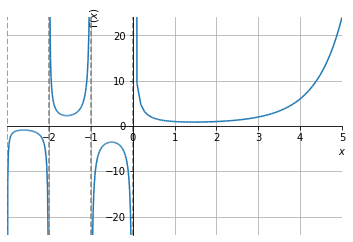
\includegraphics[width=0.7\textwidth]{cap_edolcv/dados/fig_edolcv_fg/fig}
  \caption{Esboço do gráfico da função gama $\Gamma(x)$.}
  \label{fig:edolcv_fg}
\end{figure}

\begin{obs} Vejamos as seguintes observações:
  \begin{enumerate}[a)]
  \item $\nexists\Gamma(0)$

    De fato, $\Gamma(0)$ não está definido pois
    \begin{equation}
      \lim_{x\to 0^-} \Gamma(x) = \lim_{x\to 0^-} \frac{\cancelto{\Gamma(1)=1}{\Gamma(x+1)}}{x} = -\infty
    \end{equation}
    e
    \begin{equation}
      \lim_{x\to 0^+} \Gamma(x) = \lim_{x\to 0^+} \frac{\cancelto{\Gamma(1)=1}{\Gamma(x+1)}}{x} = \infty
    \end{equation}

  \item $\nexists\Gamma(p)$, com $p$ inteiro negativo

    De fato, isto pode ser mostrado por indução a partir do item a) e da propriedade \eqref{eq:edolcv_fgp1}. Verifique!
  \end{enumerate}
\end{obs}

\begin{obs}
  Para números não naturais $x$, o valor de $\Gamma(x)$ só pode ser computado via técnicas de cálculo numérico. Uma das exceções, $\Gamma(\frac{1}{2})$, de fato
  \begin{align}
    \Gamma\left(\frac{1}{2}\right) &= \int_0^\infty z^{\frac{1}{2}-1}e^{-z}\,dz\\
                                   &= \int_0^\infty \frac{e^{-z}}{\sqrt{z}}\,dz
  \end{align}
  Fazendo a substituição $u=\sqrt{z}$, temos $\displaystyle du = \frac{dz}{2\sqrt{z}} = \frac{dz}{2u}$, obtemos
  \begin{align}
    \Gamma\left(\frac{1}{2}\right) &= \int_0^\infty \frac{e^{-u^2}}{u}\cdot 2u\,du \\
                                   &= 2\int_0^\infty e^{-u^2}\,du \\
                                   &= \int_{-\infty}^\infty e^{-u^2}\,du
  \end{align}
  Esta última é a conhecida integral de Gauss, a qual tem valor
  \begin{equation}
    \int_{-\infty}^\infty e^{-u^2}\,du = \sqrt{\pi}.
  \end{equation}]
  Logo, concluímos que
  \begin{equation}
    {\color{blue}\Gamma\left(\frac{1}{2}\right) = \sqrt{\pi}}.
  \end{equation}
\end{obs}

\subsection{Função beta}

A \emph{função beta} (ou, integral de Euler de primeiro tipo) é definida por
\begin{equation}
  {\color{blue}B(x,y) = \int_0^1 z^{x-1}(1-z)^{y-1}\,dz},
\end{equation}
para quaisquer números reais positivos $x$ e $y$.

Sua relação com a função gama é dada por
\begin{equation}\label{eq:edolcv_bg}
  {\color{blue}B(x,y) = \frac{\Gamma(x)\Gamma(y)}{\Gamma(x+y)}}.
\end{equation}
De fato, temos
\begin{align}
  \Gamma(x)\Gamma(y) &= \int_0^\infty u^{x-1}e^{-u}\,du\cdot\int_0^\infty v^{y-1}e^{-v}\,dv \\
                     &= \int_{v=0}^\infty\int_{u=0}^\infty u^{x-1}v^{y-1}e^{-(u+v)}\,du\,dv
\end{align}
Fazendo a mudança de variáveis $u=zt$ e $v=z(1-t)$, temos a jacobiana
\begin{align}
  J(u,v) &=
           \begin{vmatrix}
             \frac{\p u}{\p z} & \frac{\p u}{\p t}\\
             \frac{\p v}{\p z} & \frac{\p v}{\p t}
           \end{vmatrix}\\
         &= \begin{vmatrix}
           t & z\\
           (1-t) & -z
         \end{vmatrix}\\
         &= -z.
\end{align}
Logo,
\begin{align}
  \Gamma(x)\Gamma(y) &= \int_{z=0}^\infty\int_{t=0}^1 (zt)^{x-1}[z(1-t)]^{y-1}e^{-[zt+z(1-t)]}\,|J(u,v)|\,dt\,dz\\
                     &= \int_{z=0}^\infty z^{x+y-1}e^{-z}\,dz\cdot \int_{t=0}^1 t^{x-1}(1-t)^{y-1}\,dt\\
                     &= \Gamma(x+y) B(x,y),
\end{align}
o que nos fornece \eqref{eq:edolcv_bg}.

\begin{ex}
  \begin{equation}
    B\left(\frac{1}{2}, \frac{1}{2}\right) = \pi.
  \end{equation}
  De fato, de \eqref{eq:edolcv_bg}, temos
  \begin{align}
    B\left(\frac{1}{2}, \frac{1}{2}\right) &= \frac{\Gamma\left(\frac{1}{2}\right)\Gamma\left(\frac{1}{2}\right)}{\Gamma\left(\frac{1}{2}+\frac{1}{2}\right)}\\
                                           &= \frac{\sqrt{\pi}\sqrt{\pi}}{\Gamma(1)}\\
                                           &= \pi.
  \end{align}
\end{ex}

Para $n$ e $m$ números naturais não nulos, a propriedade \eqref{eq:edolcv_bg} mostra que a função beta guarda a seguinte relação com os coefientes binomiais
\begin{equation}\label{eq:edolcv_fgcb}
  {\color{blue}B(n,m) = \frac{n+m}{nm}\cdot \frac{1}{\binom{n+m}{n}}},
\end{equation}
onde no denominador do último termo temos o coeficiente binomial
\begin{equation}
  \binom{n+m}{n} = \frac{(n+m)!}{n!(n+m-n)!} = \frac{(n+m)!}{n!m!}.
\end{equation}
De fato, \eqref{eq:edolcv_fgcb} decorre de \eqref{eq:edolcv_bg}, pois
\begin{align}
  B(n,m) &= \frac{\Gamma(n)\Gamma(m)}{\Gamma(n+m)} \\
         &= \frac{(n-1)!(m-1)!}{(n+m-1)!}\\
         &= \frac{n!m!}{(n+m)!}\frac{n+m}{nm}\\
         &= \frac{n+m}{nm}\cdot\frac{1}{\frac{(n+m)!}{n!m!}}\\
         &= \frac{n+m}{nm}\cdot \frac{1}{\binom{n+m}{n}}.
\end{align}

\emconstrucao

\subsection*{Exercícios resolvidos}

\emconstrucao

\subsection*{Exercícios}

\emconstrucao

\section{Funções de Bessel}\label{cap_edolcv_sec_fbessel}

\emconstrucao

\subsection*{Exercícios resolvidos}

\emconstrucao

\subsection*{Exercícios}

\emconstrucao